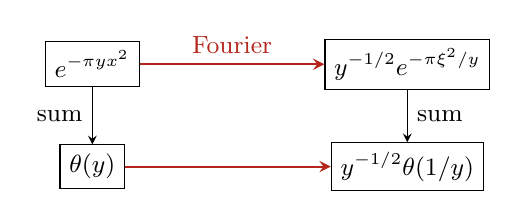
\begin{tikzpicture}[>=stealth,font=\small]
\node[draw] (a) at (0,0) {$e^{-\pi yx^2}$};
\node[draw] (b) at (4,0) {$y^{-1/2}e^{-\pi\xi^2/y}$};
\node[draw] (c) at (0,-1.3) {$\theta(y)$};
\node[draw] (d) at (4,-1.3) {$y^{-1/2}\theta(1/y)$};
\draw[->,BrickRed,thick] (a)--node[above] {Fourier}(b);
\draw[->] (a)--node[left] {sum}(c);
\draw[->] (b)--node[right] {sum}(d);
\draw[->,BrickRed,thick] (c)--(d);
\end{tikzpicture}
